\section{Kreisel} % vorläufiger Name

In dem zweiten Teilversuch  soll das Trägheitsmoment eines schweren, symmetrischen Kreisels bestimmt werden.
Dazu wird es zuerst direkt durch die geometrische Form berechnet und dann mit Hilfe der Präzession graphisch ermittelt.

\subsection{Methoden}

	\subsubsection{Aufbau}
	
	Ein Kreisel besteht aus einer Metallkugel, einer Verbindungsstange und einem an dieser verschiebbaren Gewicht.
	Der Kreisel wird auf ein Luftkissen annähernd reibungsfrei gelagert.
	Zudem wird so der Unterstützungspunkt im Kugelmittelpunkt gehalten.
	Zunächst stehe der Kreisel aufrecht.
	Die Kugel wird nun tangential mit Druckluft angeblasen, bis der Kreisel stabil rotiert.
	Der Kreisel wird in etwa um den Winkel $\frac{\pi}{4}$ gekippt und präzessiert nun zusätzlich um die Senkrechte.
	Für eine weitere Stabilisierung kann der Kreisel einmal am Finger entlang geleitet werden, um unregelmäßige Bewegungen weitgehend zu vermeiden.
	
	Ein Stroboskoplicht wird eingeschaltet und auf eine bestimmte Frequenz eingestellt.
	Durch einen kleinen weißen Punkt auf der Kugel kann die Rotation des Kreisels mit der Frequenz des Stroboskoplichtes synchronisiert werden.
	Dies ist dann erreicht, wenn sich der Punkt scheinbar nicht mehr bewegt.
	Dabei kann eine feine Abstimmung durch Variation des Abstandes und des Winkels der Druckluftdüse zu der Metallkugel erreicht werden.
	
	\subsubsection{Komplikationen}
	
	Der erste verwendete Kreisel war nicht ganz stabil und die Präzessionsbewegung wies stets nach kurzer Zeit unruhige Bewegungen auf.
	Das kommt wahrscheinlich von einer Unwucht, also einer Deformation des Kreisels.
	
	Der Kreisel ist beim Abbremsen von einer hohen Frequenz von über \SI{3500}{\hertz} von der Platform geflogen.
	Bei allen weiteren Messungen wurde die Kugel immer erst mit Druckluft abgebremmst und senkrecht aufgerichtet, bevor sie gestoppt wurde.
	
	\subsubsection{Unsicherheiten}
	
<<<<<<< HEAD
	Das Stroboskoplicht sei relativ zur Frequenz auf $1\%$ ungenau.
	Also $u(f) = 0,01 f$.
	
	Die Kugel wurde mit Hilfe einer Schieblehre vermessen.
	Diese hatte eine ablesbare Unsicherheit von $u(r_k) =\frac{1}{50}\si{\milli\meter}$.
	Man konnte die Kugel durch die Schieblehre gleiten lassen, um so den größtmöglichen Abstand auf der Kugeloberfläche, also den Durchmesser zu erhalten.
	
	Die benutzten Massen wurden mit einer digitalen Waage gewogen.
	Da sie zwei Nachkommastellen anzeigen konnte, folgt eine Ungenauigkeit von $u(m_k) = \frac{0,01}{2\sqrt{3}}\si{g}$
	
	Das für die Kraftmessungen benutzte Newtonmeter konnte auf \SI{0,01}{\newton} genau abgelesen werden.
	Die Unsicherheit beträgt somit $u(F) = \frac{0,01}{2\sqrt{6}} \si{newton}$.
	
	Für die Zeitmessung mit einer Stoppuhr wird die Reaktions- $u(t_R) = \frac{0,1}{2\sqrt6}\si{\second}$ und die digitale Ungenauigkeit $u(t_D) = \frac{0,01}{2\sqrt3}\si{\second}$ miteinander kombiniert.
	Es folgt $u(t) \approx \SI{0,0206}{\second}$\footnote{Unsicherheitsrechnung siehe Gl. (\ref{eq:unc_t}) im Anhang.}.
	
	Für sich fortpflanzende Unsicherheiten wird die folgende Formel verwendet.
	\begin{equation}
		\label{eq:unc_combined}
		u(a) = \sqrt{\sum_{k=1}^{n} \pdv{a}{x_k} u(x_k)}
	\end{equation}
	Für kombinierte Unsicherheiten folgt aus dieser $u(b) = \sqrt{\sum_{k=1}^n u(b_k)^2}$.
	Bei graphisch ermittelten Werten wird die Unsicherheit automatisch errechnet\footnote{Z. B. im Programm SciDaVis beim erstellen eines Fits.}.
=======
		%TODO
		Zur Berechnung der Unsicherheiten für die gemessenen und ermittelten Werte dient folgende Formel: 
		\begin{equation*}
		u(s) = \pm \sqrt{\sum_{k=0}^{N}\left( \frac{\partial f}{\partial x_i}u(x_i)\right) ^2}. 
		\end{equation*}
>>>>>>> 3f5ad67e9305bed0e93a2f8e917dbeff04d1a0d9

\subsection{Messung}
	
	Der Kugeldurchmesser wurde fünf mal mit der Schieblehre vermessen.
	Es ergibt sich ein Kugelradius $r_k = \SI{2,5292 +- 0,0145}{\centi\meter}$.
	Die Kugel hat ein Gewicht von $m_r = \SI{511,08 +- 0,003}{g}$.
	
	Die Kugel hat ein Trägheitsmoment von $J = J_1 + J_2$.
	Dabei war angegeben, dass $J_1 = \SI{15}{g\,\centi\meter\squared}$.
	Das Trägheitsmoment der massiven Metallkugel mit Masse $m_k$ und Radius $r_k$ ist $J_2 = \frac{2}{5} m_k r_k^2 \approx \SI{1307,72 +- 15,01}{g\,\centi\meter\squared}$ und somit folgt ein gesammtes Trägheitsmoment von $J = \SI{1322,72 +- 15,01}{g\,\centi\meter\squared}$\footnote{Unsicherheitsrechnung siehe Gl. (\ref{eq:unc_traeg}) im Anhang.}.
	
	
	Nun werden für die drei unterschiedlichen Positionen der Zusatzmasse die Kräfte ermittelt.
	In Tab. \ref{tab:mess_kraefte} sind die Mittelwerte mit ihren Unsicherheiten aufgelistet.
	\begin{table}[ht]
		\caption{Gemessene Kräfte des Kreisels am äußeren Rand der Stange. Zusätzlich das daraus resultiernde Drehmoment.}
		\centering
		\label{tab:mess_kraefte}
		\begin{tabular}{c|S|S}
			{Position Zusatzgewicht} & {Kraft} & {Drehmoment}\\
			\hline
			{Gewicht außen} & {\SI{0,222 +- 0,008}{\newton}} & \SI{2,539 +- 0,096}{\newton\,\centi\meter}\\
			{Gewicht mittig} & {\SI{0,202 +- 0,004}{\newton}} & \SI{2,310 +- 0,051}{\newton\,\centi\meter}\\	
			{Gewicht innen} & {\SI{0,16 +- 0,0}{\newton}} & \SI{1,830 +- 0,002}{\newton\,\centi\meter}\\
			
		\end{tabular}
	\end{table}
	Je weiter innen das Zusatzgewicht liegt, desto kleiner ist auch die resultierende Kraft.
	Die Länge vom Kugelmittelpunkt bis zum Newtonmeteransatzpunkt kann durch $l = L - h + r_k$ angegeben.
	Dabei ist $L = \SI{9,214 +- 0,004}{\centi\meter}$ die gesammte Stablänge (bis zum Gewinde) und $h = \SI{0,306 +- 0,002}{\centi\meter}$ die Diche des Halteringes am Ende des Stabes.
	Es folgt $l = \SI{11,44 +- 0,02}{\centi\meter}$\footnote{Es handelt sich um eine kombinierte Unsicherheit, Rechnung im Anhang Gl. (\ref{eq:unc_length}).}.
	
	Aus den Kräften $F$ und der Läge $l$ kann nun mit der Beziehung $amg = lF$ das Drehmoment für die drei Positionen des Zusatzgewichtes berechnet werden.
	Die zugehörigen Werte finden sich in Tab. \ref{tab:mess_kraefte}.
	
	Bei der Präzession wird graphisch ausgewertet.
	Dazu werden die erhaltenen Werte $T_P$ gegen $\omega = 2\pi f$ ($u(\omega) = 2\pi u(f)$) aufgetragen.
	\begin{figure}[ht]
		\centering
		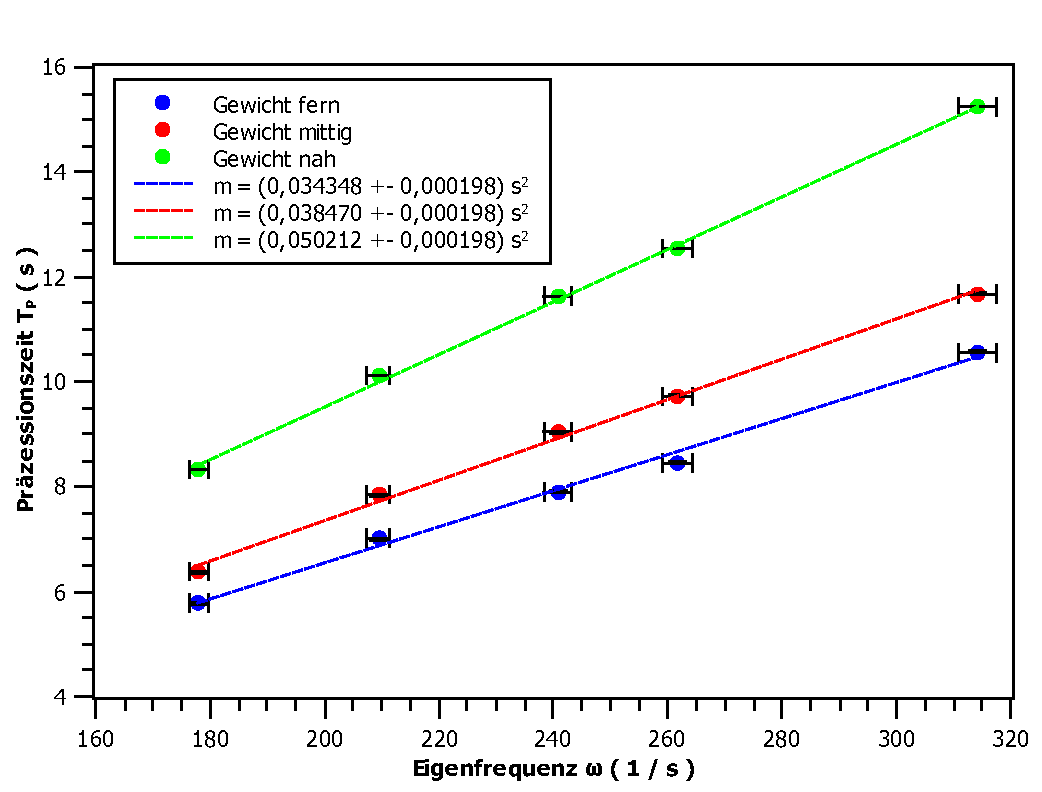
\includegraphics[width=\textwidth]{kreisel_wT_multi.pdf}
		\caption{Darstellung der Präzessionszeit gegen die Eigenfrequenz des Kreisel. Die drei unterschiedlichen Gewichtspositionen sind farblich gekennzeichnet.}
		\label{abb:Tw-multi}	
	\end{figure}
	Wie in Abb. \ref{abb:Tw-multi} zu erkennen ist, erhält man durch Linearisierung der Datenpunkte\footnote{Programm: SciDaVis; Algorithmus: kleinste Quadrate} für jede Gewichtsposition eine Steigung, im folgenden $m$ genannt.
	Dabei fällt auf, dass die Steigung größer ist, je näher das Gewicht an der Kugel ist.
	
	Nun werden die Punkte $(\frac{1}{m}, lF)$ in ein weiteres Diagramm gesetzt und ebenso linearisiert.
	\begin{figure}[ht]
		\centering
		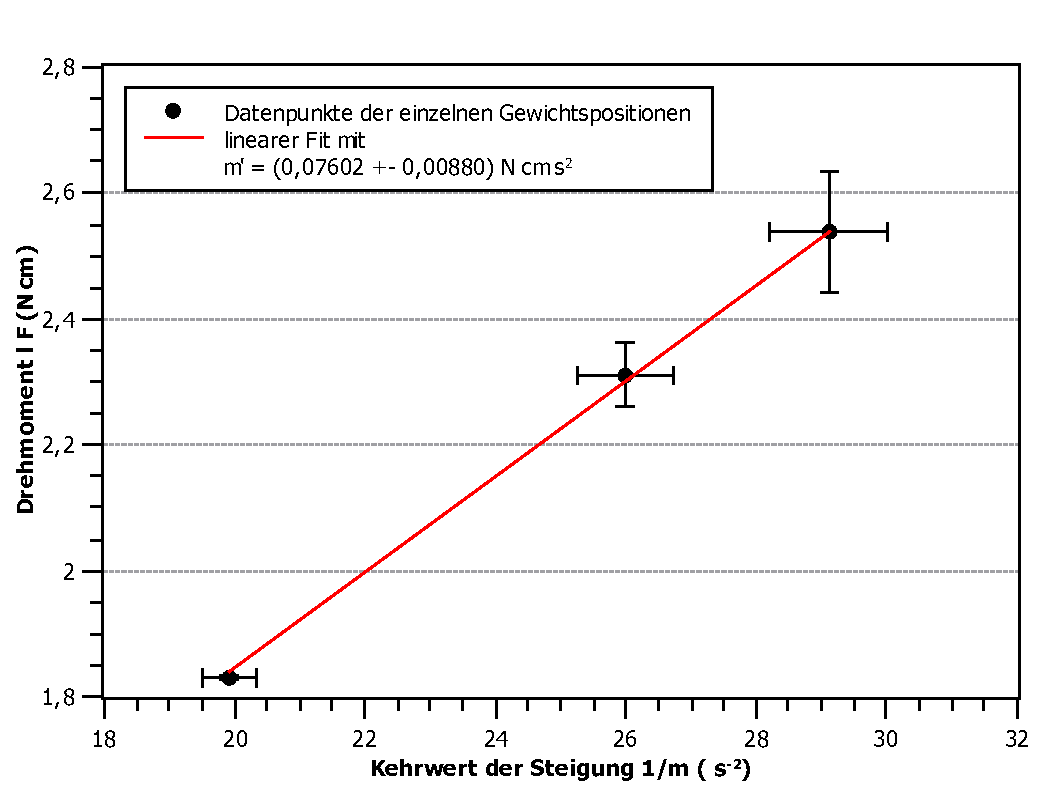
\includegraphics[width=\textwidth]{kreisel_gewichte.pdf}
		\caption{Darstellung und Linearisierung der drei Datensätze für unterschiedliche Gewichtspositionen. Es sei anzumerken, dass die Steigung die Einheit $\si{\newton\,\centi\meter\,\second\squared} = 10^5\cdot \si{g\,\centi\meter^2}$ hat.}
		\label{abb:gewichte}	
	\end{figure}
	Für die dort erhaltene Steigung gilt gerade eben $m' = \SI{0,07602 +- 0,00880}{\newton\,\centi\meter\,\second\squared} = 2\pi J$, bzw. umgestellt $J = \frac{m'}{2\pi}$.
	Nach beachten der Einheiten folgt:
	\begin{equation}
		J = \frac{m'}{2\pi} \approx \SI{1209,8 +- 140,1}{g\,\centi\meter\squared}
	\end{equation}
	

\subsection{Zusammenfassung}

Es wurde das Trägheitsmoment eines schweren, symmetrischen Kreisels auf zwei Arten ermittelt.
Zum einen wurde dieses durch die geometrische Form direkt berechnet.
Zum anderen konnte es durch die Präzession bei verschiedenen Positionen eines Zusatzgewichtes bestimmt werden.

Vergleicht man das graphisch ermittelte Trägheitsmoment mit dem geometrisch errechneten, so liegt letzteres in einem guten Vertrauensbereich.
Andersherum liegt aber der graphisch ermittelte Wert weit außerhalb des Vertrauensbereich des errechneten Wertes.


\subsection{Schlussfolgerung}

Die relative Unsicherheit des graphisch ermittelten Trägheitsmoment ist mit $10\%$ recht hoch.
Um weitere Übereinstimmungen zu erhalten, muss das Experiment ggf. noch einmal wiederholt werden, um einen schärferen graphischen Wert zu bekommen.
Dabei wäre es besonders wichtig, die Präzessionszeit über mehrere Perioden zu bestimmen und dabei die Eigenfrequenz des Kreisels konstant zu halten.
Das könnte z. B. durch eine längere Einpendelzeit vor der Messung eingebracht werden.

\subsection{Anhang}

\begin{equation}
	\label{eq:unc_t}
	u(t) = \sqrt{u(t_R)^2 + u(t_D)^2} \approx \SI{0,020615}{\second}
\end{equation}

\begin{align}
	\label{eq:unc_traeg}
	u(J) = u(J_2) &= \frac{2}{5} \sqrt{\left( \pdv{m_k r_k^2}{m_k} u(m_k)\right) ^2 + \left( \pdv{m_k r_k^2}{r_k} u(r_k)\right) ^2}\\
	&= \frac{2}{5} \sqrt{(r_k^2 u(m_k))^2 + (2r_k m_k u(r_k))^2} \approx \SI{15,010472}{g\,\centi\meter\squared}
\end{align}

\begin{equation}
	\label{eq:unc_length}
	u(l) = \sqrt{u(L)^2 + u(r_k)^2 + u(h)^2} \approx \SI{0,015215}{\centi\meter}
\end{equation}

\begin{equation}
	\label{eq:unc_traeg2}
	u(J) = \frac{1}{2\pi} \pdv{m'}{m'} u(m') = \frac{u(m')}{2\pi}
\end{equation}
